% ============================================================================
%  Impact of Reconstruction Errors on Connectome Graph Analysis
%  Beamer presentation — BANC dataset experiments (EM1 missed synapses,
%  EM2 false synapses).  One idea per slide, larger fonts, takeaway boxes.
%
%  Figures:  python make_figures.py
%  Compile:  pdflatex main.tex  (twice for page refs)
% ============================================================================
\documentclass[aspectratio=169,11pt]{beamer}

% ---- encoding & fonts ------------------------------------------------------
\usepackage[utf8]{inputenc}
\usepackage[T1]{fontenc}
\usepackage{amsmath,amssymb}
\usepackage{graphicx}
\graphicspath{{figures/}}
\usepackage{booktabs}
\usepackage{xcolor}
\usepackage{tikz}
\usetikzlibrary{arrows.meta,positioning}

% ---- palette ---------------------------------------------------------------
\definecolor{navy}{RGB}{22,41,66}
\definecolor{accent}{RGB}{11,110,153}    % blue  (missed synapses)
\definecolor{accentb}{RGB}{196,69,29}    % orange (false synapses)
\definecolor{baselinec}{RGB}{154,165,177}
\definecolor{boxlight}{RGB}{242,246,250}
\definecolor{boxtitle}{RGB}{22,41,66}
\definecolor{okgreen}{RGB}{90,143,78}
\definecolor{warnc}{RGB}{217,164,65}

% ---- beamer look -----------------------------------------------------------
\setbeamercolor{structure}{fg=navy}
\setbeamercolor{frametitle}{fg=navy}
\setbeamercolor{normal text}{fg=navy!90}
\setbeamercolor{itemize item}{fg=accent}
\setbeamercolor{itemize subitem}{fg=accent!70}
\setbeamercolor{block title}{fg=white,bg=boxtitle}
\setbeamercolor{block body}{bg=boxlight}
\setbeamertemplate{navigation symbols}{}
\setbeamertemplate{blocks}[rounded][shadow=false]
\setbeamertemplate{block body begin}{\raggedright}
\setbeamertemplate{frametitle}{%
  \vskip4pt
  \noindent\usebeamerfont{frametitle}\insertframetitle\par
  \vskip2pt
  {\color{accent}\hrule height1.2pt}
  \vskip3pt
}
\setbeamertemplate{footline}{%
  \leavevmode\hbox{%
    \begin{beamercolorbox}[wd=.30\paperwidth,ht=2.4ex,dp=1ex,left]{author in head/foot}%
      \hspace*{0.35cm}\scriptsize\color{baselinec}BANC Dataset
    \end{beamercolorbox}%
    \begin{beamercolorbox}[wd=.40\paperwidth,ht=2.4ex,dp=1ex,center]{title in head/foot}%
      \scriptsize\color{baselinec}Reconstruction Errors on Connectome Analysis
    \end{beamercolorbox}%
    \begin{beamercolorbox}[wd=.30\paperwidth,ht=2.4ex,dp=1ex,right]{date in head/foot}%
      \scriptsize\color{baselinec}\insertframenumber{} / \inserttotalframenumber\hspace*{0.35cm}
    \end{beamercolorbox}}%
}

% takeaway box: colored strip at the bottom of a results slide
\newcommand{\takeaway}[2][okgreen]{%
  \vskip6pt
  \begin{beamercolorbox}[rounded=true,sep=6pt,wd=\textwidth]{block body}
    {\color{navy}\textbf{Takeaway:}~#2}
  \end{beamercolorbox}%
}

\begin{document}

% ============================================================================
% Slide 1 — Title
% ============================================================================
{
\setbeamertemplate{footline}{}
\begin{frame}[plain]
  \begin{tikzpicture}[remember picture,overlay]
    \fill[navy] (current page.north west) rectangle ([yshift=-3.4cm]current page.north east);
    \fill[accent] ([yshift=-3.4cm]current page.north west) rectangle ([yshift=-3.62cm]current page.north east);
  \end{tikzpicture}
  \vspace*{1.15cm}
  {\color{white}\LARGE\bfseries Impact of Reconstruction Errors\\[6pt] on Connectome Graph Analysis}
  \vspace{1.1cm}

  {\large\color{navy!80}Experimental Analysis of Missed Synapses and False Synapses}
  \vspace{1.6cm}

  
\begin{tikzpicture}
    \node[draw=accent, rounded corners=3pt, fill=accent!8, minimum width=3.6cm,
          minimum height=0.7cm, font=\normalsize\color{navy}] {BANC Dataset};
  \end{tikzpicture}
  \vfill
  {\footnotesize\color{baselinec}Neuron- and synapse-resolved connectome simulation study $\cdot$ 10 error rates $\cdot$ 5 trials each}
\end{frame}
}

% ============================================================================
% Slide 2 — The problem
% ============================================================================
\begin{frame}{The Problem}
\begin{block}{Connectomes are reconstructed from noisy imaging data}
  \footnotesize
  Every neuron and every synapse in a connectome is the output of an automated
  segmentation / synapse-detection pipeline --- and pipelines make mistakes.
\end{block}

\vskip2pt
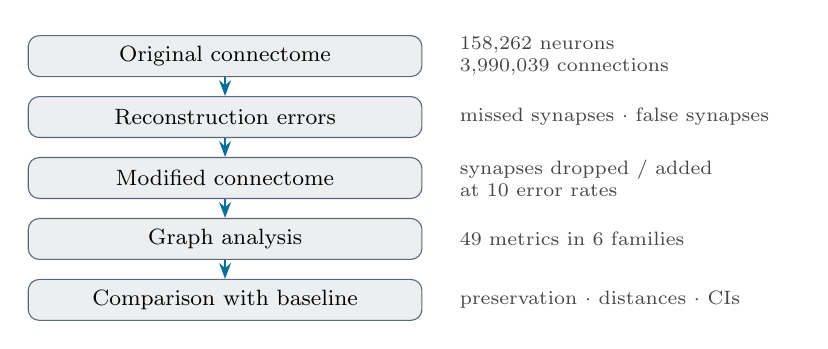
\begin{tikzpicture}[
  box/.style={draw=navy!70, fill=navy!8, rounded corners=4pt,
              minimum width=5.0cm, minimum height=0.52cm, font=\footnotesize},
  arr/.style={-{Stealth[length=2mm]}, thick, color=accent},
  note/.style={font=\scriptsize, color=gray!55!black, text width=4.2cm, align=left}
]
  \node[box] (a) {Original connectome};
  \node[note, right=0.35cm of a] (ca) {158{,}262 neurons\\ 3{,}990{,}039 connections};
  \node[box, below=0.24cm of a] (b) {Reconstruction errors};
  \node[note, right=0.35cm of b] (cb) {missed synapses $\cdot$ false synapses};
  \node[box, below=0.24cm of b] (c) {Modified connectome};
  \node[note, right=0.35cm of c] (cc) {synapses dropped / added\\ at 10 error rates};
  \node[box, below=0.24cm of c] (d) {Graph analysis};
  \node[note, right=0.35cm of d] (cd) {49 metrics in 6 families};
  \node[box, below=0.24cm of d] (e) {Comparison with baseline};
  \node[note, right=0.35cm of e] (ce) {preservation $\cdot$ distances $\cdot$ CIs};
  \draw[arr] (a) -- (b);
  \draw[arr] (b) -- (c);
  \draw[arr] (c) -- (d);
  \draw[arr] (d) -- (e);
\end{tikzpicture}

\vskip4pt
\begin{block}{Question}
  \footnotesize
  How much do these errors distort the results of graph analysis --- and do
  different error types distort it differently?
\end{block}
\end{frame}

% ============================================================================
% Slide 3 — Research questions
% ============================================================================
\begin{frame}{Research Questions}
\begin{itemize}
  \item \textbf{Direct effect.} How do total synapses and connections change
        as the error rate grows?
        \vskip2pt {\footnotesize\color{gray} Expected: proportional to the rate --- but by how much for edges?}
  \item \textbf{Structural effect.} Are global properties (connectivity,
        reciprocity, hub ranking) preserved, or do they degrade?
        \vskip2pt {\footnotesize\color{gray} Does the coarse wiring plan survive 20\% error?}
  \item \textbf{Comparative effect.} Which error type --- missed synapses
        (false negatives) or false synapses (false positives) --- is more
        disruptive at the same nominal rate?
        \vskip2pt {\footnotesize\color{gray} Same rate, different fingerprints?}
\end{itemize}

\vskip6pt
\begin{block}{Deliverable}
  \footnotesize
  A data-backed comparison of two error models on the BANC connectome:
  what degrades first, what survives, and how to tell the models apart.
\end{block}
\end{frame}

% ============================================================================
% Slide 4 — Dataset & baseline
% ============================================================================
\begin{frame}{Dataset and Baseline}
\begin{columns}[c]
  \begin{column}{0.55\textwidth}
    \footnotesize\renewcommand{\arraystretch}{1.6}
    \begin{tabular}{@{}ll@{}}
      \toprule
      \textbf{Dataset} & BANC --- \emph{D.~melanogaster}\\
                       & brain + nerve cord\\
      \midrule
      \textbf{Neurons} & 158{,}262\\
      \textbf{Connections} & 3{,}990{,}039\\
      \textbf{Synapses} & 23{,}556{,}214\\
      \midrule
      \textbf{Reciprocity} & 0.1299\\
      \textbf{Giant SCC} & 139{,}405 vertices\\
      \textbf{Mean edge weight} & 5.90 synapses\\
      \bottomrule
    \end{tabular}
  \end{column}
  \begin{column}{0.42\textwidth}
    \begin{block}{Baseline role}
      \small
      The original graph is the \emph{ground truth}.  Every experiment
      perturbs this graph, re-runs the analyses, and compares the result
      with the baseline --- a controlled, paired design.
    \end{block}
    \begin{block}{Why BANC?}
      \small
      A full adult brain + nerve cord connectome: large enough to be
      realistic, small enough to run 100 perturbation trials.
    \end{block}
  \end{column}
\end{columns}
\end{frame}

% ============================================================================
% Slide 5 — Error model 1
% ============================================================================
\begin{frame}{Error Model 1: Missed Synapses (False Negatives)}
\begin{columns}[c]
  \begin{column}{0.42\textwidth}
    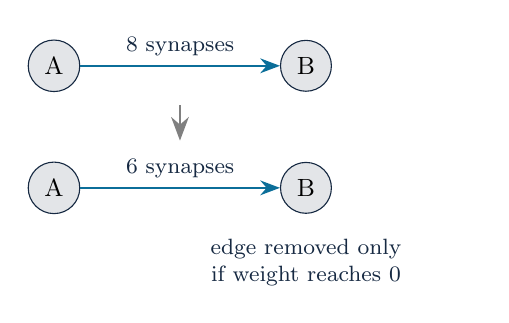
\begin{tikzpicture}[
      neuron/.style={circle, draw=navy, fill=navy!12, minimum size=0.55cm, font=\small},
      syn/.style={font=\footnotesize, color=navy},
      arr/.style={-{Stealth[length=2.5mm]}, thick, color=accent},
      darr/.style={-{Stealth[length=3mm]}, thick, color=gray}
    ]
      \node[neuron] (A1) at (0,0) {A};
      \node[neuron] (B1) at (3.2,0) {B};
      \draw[arr] (A1) -- node[syn,above]{8 synapses}(B1);
      \draw[darr] (1.6,-0.5) -- (1.6,-0.95);
      \node[neuron] (A2) at (0,-1.55) {A};
      \node[neuron] (B2) at (3.2,-1.55) {B};
      \draw[arr] (A2) -- node[syn,above]{6 synapses}(B2);
      \node[syn, below=0.2cm of B2, text width=4.2cm, align=center]
        {edge removed only if weight reaches 0};
    \end{tikzpicture}
  \end{column}
  \begin{column}{0.55\textwidth}
    \begin{block}{Mechanism}
      \footnotesize
      Each synapse survives independently with probability $1-r$
      (binomial sampling).  The edge weight becomes the number of
      surviving synapses.
    \end{block}
    \begin{block}{Consequences}
      \footnotesize
      \begin{itemize}
        \item Synapse count drops $\approx r$ (linear).
        \item Edge count drops \emph{slowly}: an edge survives while at
              least one synapse remains.
        \item Topology (which neurons connect) is largely preserved.
        \item $r$ swept over 10 rates: 0 -- 20\%; seeded, 5 trials per rate.
      \end{itemize}
    \end{block}
  \end{column}
\end{columns}
\end{frame}

% ============================================================================
% Slide 6 — Error model 2
% ============================================================================
\begin{frame}{Error Model 2: False Synapses (False Positives)}
\begin{columns}[c]
  \begin{column}{0.42\textwidth}
    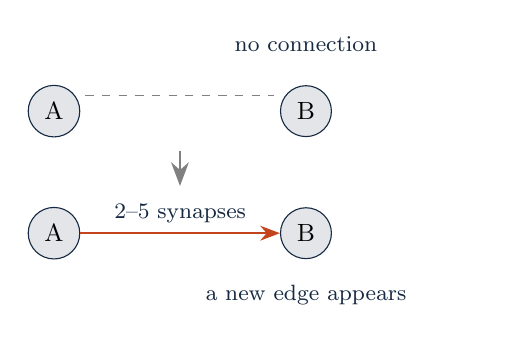
\begin{tikzpicture}[
      neuron/.style={circle, draw=navy, fill=navy!12, minimum size=0.55cm, font=\small},
      syn/.style={font=\footnotesize, color=navy},
      arr/.style={-{Stealth[length=2.5mm]}, thick, color=accentb},
      darr/.style={-{Stealth[length=3mm]}, thick, color=gray},
      none/.style={dashed, color=gray}
    ]
      \node[neuron] (A1) at (0,0) {A};
      \node[neuron] (B1) at (3.2,0) {B};
      \draw[none] (0.4,0.2) -- (2.8,0.2);
      \node[syn, above=0.3cm of B1] {no connection};
      \draw[darr] (1.6,-0.5) -- (1.6,-0.95);
      \node[neuron] (A2) at (0,-1.55) {A};
      \node[neuron] (B2) at (3.2,-1.55) {B};
      \draw[arr] (A2) -- node[syn,above]{2--5 synapses}(B2);
      \node[syn, below=0.2cm of B2, text width=4.2cm, align=center]
        {a new edge appears};
    \end{tikzpicture}
  \end{column}
  \begin{column}{0.55\textwidth}
    \begin{block}{Mechanism}
      \footnotesize
      $k = r \times \text{(edge count)}$ artificial connections are injected
      between neuron pairs with \emph{no} connection; weights drawn from the
      weak-edge distribution ($\le 5$ synapses).
    \end{block}
    \begin{block}{Consequences}
      \footnotesize
      \begin{itemize}
        \item Edge count grows $\approx r$ (linear).
        \item Injected edges are \emph{weak} ($\approx$3 synapses vs.\
              baseline mean 5.9).
        \item No new strong hubs are created --- but the graph is inflated.
        \item Same 10 rates (0 -- 20\%), same seeds, 5 trials per rate.
      \end{itemize}
    \end{block}
  \end{column}
\end{columns}
\end{frame}

% ============================================================================
% Slide 7 — Experimental design
% ============================================================================
\begin{frame}{Experimental Design}
\begin{columns}[T]
  \begin{column}{0.52\textwidth}
    \footnotesize\renewcommand{\arraystretch}{1.3}
    \begin{tabular}{@{}ll@{}}
      \toprule
      \textbf{Error rates} & 0, 0.25, 0.5, 0.75, 1, 2, 5, 10, 15, 20\%\\
      \midrule
      \textbf{Trials} & 5 seeded per rate\\
      \textbf{Total runs} & 2 models $\times$ 10 rates $\times$ 5 trials\\
      \midrule
      \textbf{Metrics} & 49 in 6 analysis families\\
      \midrule
      \textbf{Runtime} & $\approx$3 min / trial ($\approx$5 h total)\\
      \bottomrule
    \end{tabular}
  \end{column}
  \begin{column}{0.46\textwidth}
    \begin{block}{Pipeline (fixed order)}
      \scriptsize
      Load $\rightarrow$ Build $\rightarrow$ Preprocess $\rightarrow$\\
      \quad\textbf{Perturb (error model)} $\rightarrow$\\
      Analyze $\rightarrow$ Statistics $\rightarrow$ Export
    \end{block}
    \begin{block}{Analysis families}
      \scriptsize
      structure $\cdot$ degree distributions $\cdot$ SCC/WCC $\cdot$
      reciprocity $\cdot$ assortativity $\cdot$ PageRank
    \end{block}
    \begin{block}{Reproducibility}
      \scriptsize
      All stochastic operations use recorded seeds; trials differ only by
      the seeded sampling.
    \end{block}
  \end{column}
\end{columns}
\end{frame}

% ============================================================================
% Slide 8 — How preservation is measured
% ============================================================================
\begin{frame}{How is Preservation Measured?}
\begin{block}{Symmetric preservation ratio}
  \footnotesize
  Every graph metric is converted to a preservation score between the
  baseline value $B$ and the perturbed value $P$:
  \[
    \mathrm{Preservation\,(\%)} = \frac{\min(B,\,P)}{\max(B,\,P)} \times 100
  \]
  A metric that does not change scores 100\%; a 20\% loss scores 80\%.
\end{block}

\vskip4pt
\begin{block}{Which metrics qualify?}
  \footnotesize
  \textbf{14 of 49} metrics have a well-defined baseline (node/edge counts,
  weights, reciprocity, assortativity, components) and enter the
  preservation analysis.  The other 35 (KS / Wasserstein distances, PageRank
  score rows) have baseline 0 --- the symmetric ratio is meaningless --- so
  they are reported as \emph{distances} instead.
\end{block}

\vskip4pt
\begin{block}{Status labels}
  \footnotesize
  Preserved $\ge$99\% $\cdot$ Minor $\ge$95\% $\cdot$ Moderate $\ge$90\% $\cdot$
  Significant $<$90\%
\end{block}
\end{frame}

% ============================================================================
% Slide 9 — Result 1: direct effects
% ============================================================================
\begin{frame}{Result 1: Direct Effects are Proportional to the Rate}
\begin{columns}[c]
  \begin{column}{0.62\textwidth}
    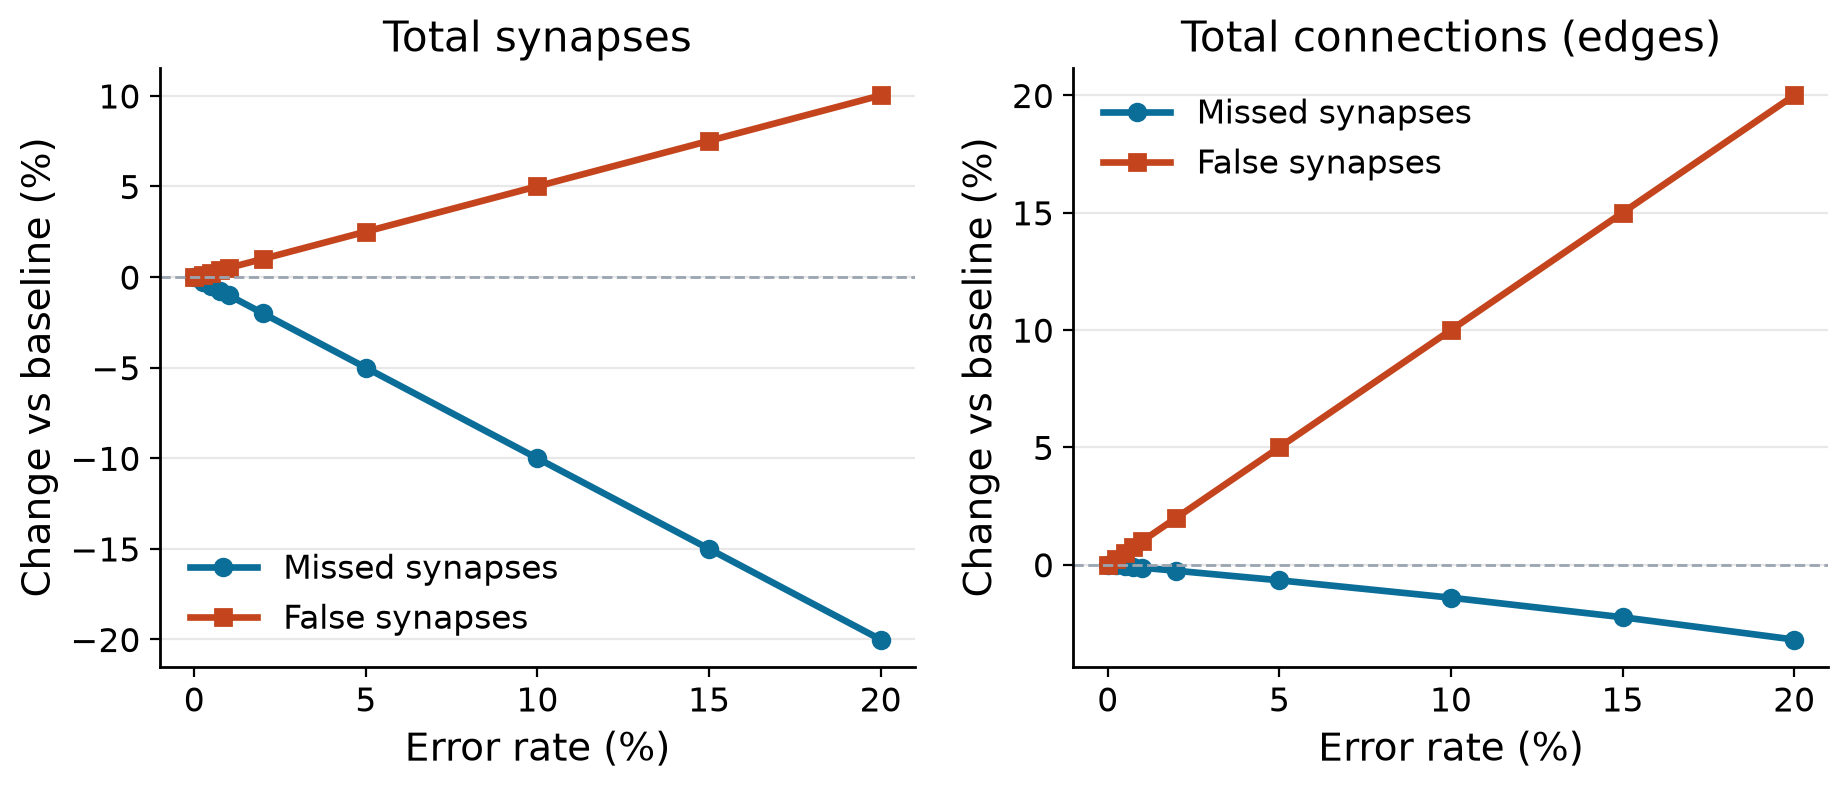
\includegraphics[width=\textwidth]{fig_primary}
  \end{column}
  \begin{column}{0.36\textwidth}
    \footnotesize
    \begin{itemize}
      \item \textbf{Missed:} synapses $-$20.0\% at 20\% rate --- exactly
            proportional; edges only $-$3.2\%.
      \item \textbf{False:} edges $+$20.0\%, synapses $+$10.0\% --- again
            proportional.
      \item Both trends are linear across all ten rates.
    \end{itemize}
  \end{column}
\end{columns}
\takeaway{Both models act exactly as calibrated: the perturbed quantity
(synapses or edges) moves in proportion to the error rate --- a clean,
predictable first-order signal.}
\end{frame}

% ============================================================================
% Slide 10 — Result 2: network organization
% ============================================================================
\begin{frame}{Result 2: The Coarse Wiring is Highly Robust}
\begin{columns}[c]
  \begin{column}{0.62\textwidth}
    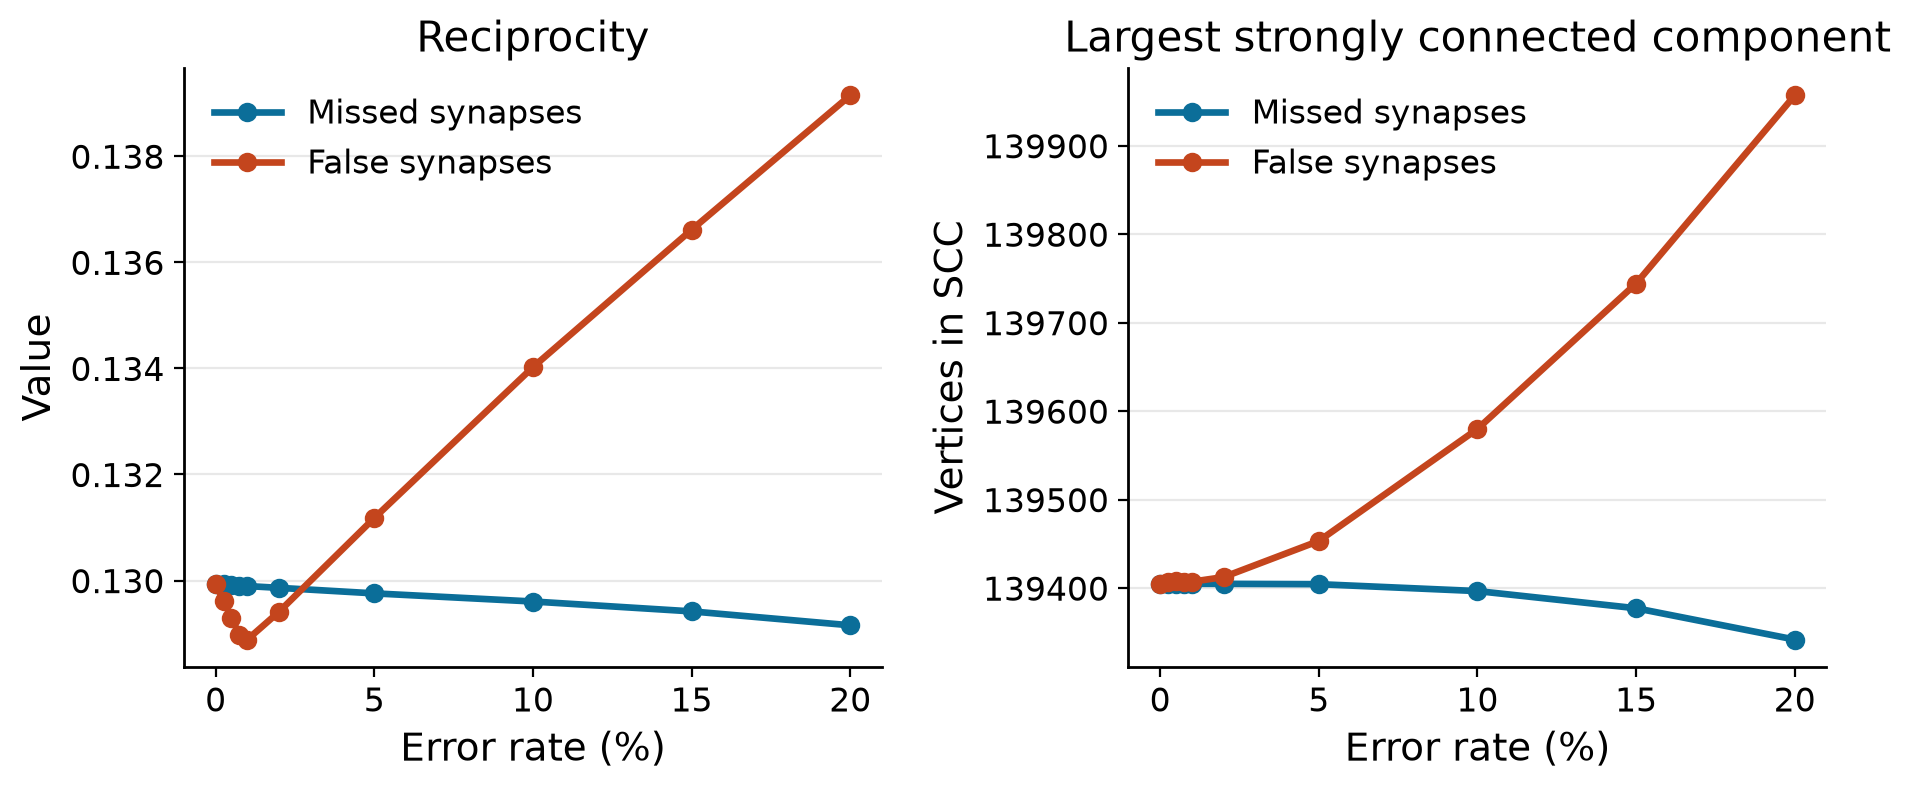
\includegraphics[width=\textwidth]{fig_organization}
  \end{column}
  \begin{column}{0.36\textwidth}
    \footnotesize
    \begin{itemize}
      \item \textbf{Giant SCC} keeps 99.95\% of vertices under missed;
            grows 0.40\% under false --- essentially unchanged.
      \item \textbf{Reciprocity} moves only $-$0.6\% (missed) / $+$7.1\%
            (false).
      \item The graph stays connected and its wiring plan survives.
    \end{itemize}
  \end{column}
\end{columns}
\takeaway{Even at 20\% error, the global architecture --- connectivity and
reciprocity --- is barely disturbed by either error type.}
\end{frame}

% ============================================================================
% Slide 11 — Result 3: PageRank
% ============================================================================
\begin{frame}{Result 3: Hub Ranking Survives, False Synapses Erode It More}
\begin{columns}[c]
  \begin{column}{0.54\textwidth}
    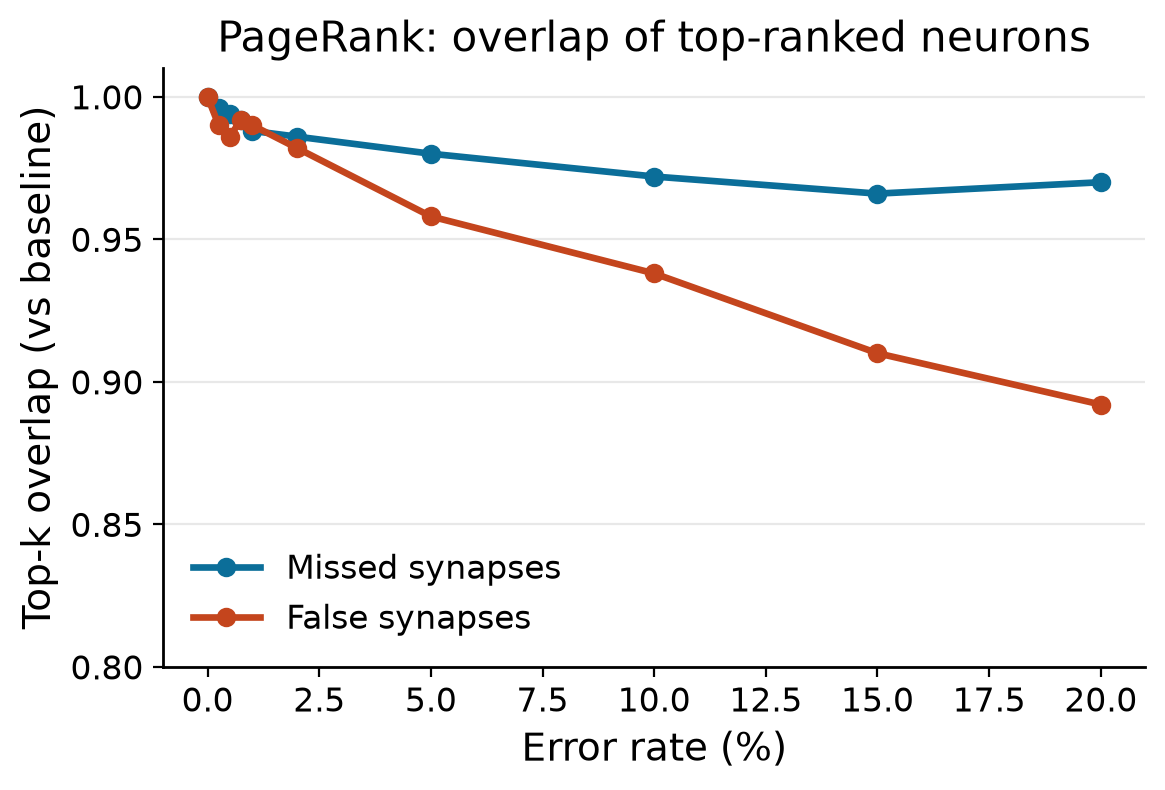
\includegraphics[width=\textwidth]{fig_pagerank}
  \end{column}
  \begin{column}{0.44\textwidth}
    \footnotesize
    \begin{itemize}
      \item \textbf{Correlation} with baseline PageRank: 0.9975 (missed) vs.\
            0.9833 (false) at 20\%.
      \item \textbf{Top-$k$ overlap} of ranked neurons: 0.970 (missed) vs.\
            0.892 (false) at 20\%.
      \item The identity of the most important neurons is largely preserved;
            injected weak edges add ranking noise without creating hubs.
    \end{itemize}
  \end{column}
\end{columns}
\takeaway{Hub ranking is robust under both models, but false synapses erode
it noticeably more (top-$k$ 0.89 vs.\ 0.97).}
\end{frame}

% ============================================================================
% Slide 12 — Result 4: degree distributions
% ============================================================================
\begin{frame}{Result 4: False Synapses Distort Degree Distributions Far More}
\begin{columns}[c]
  \begin{column}{0.62\textwidth}
    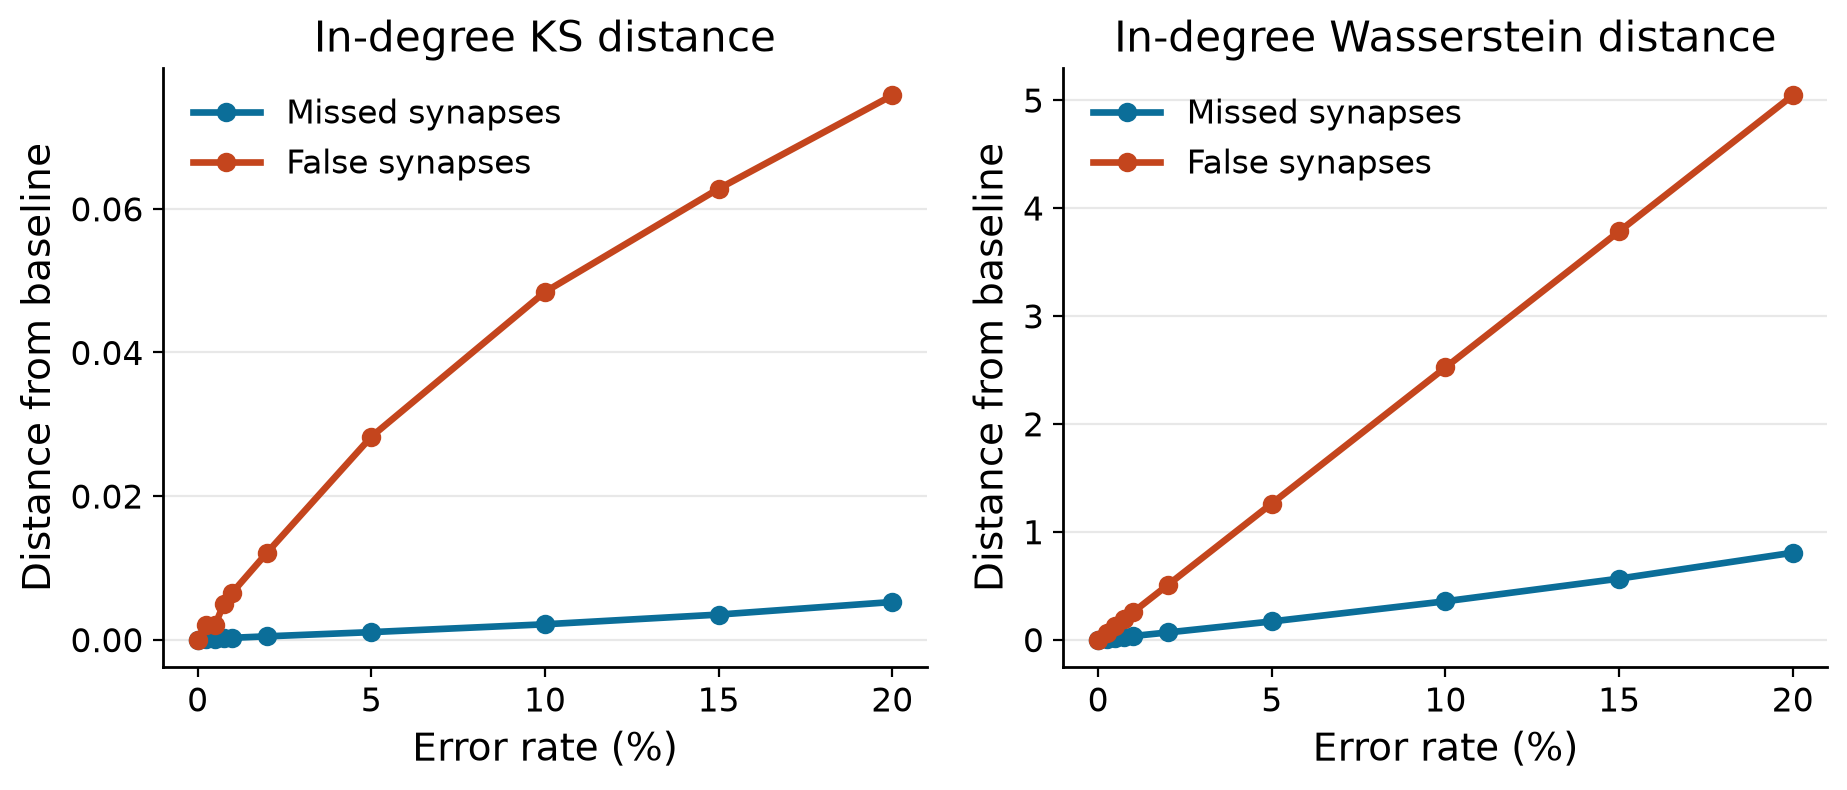
\includegraphics[width=\textwidth]{fig_degree_dist}
  \end{column}
  \begin{column}{0.36\textwidth}
    \footnotesize
    \begin{itemize}
      \item In-degree \textbf{KS distance} at 20\%: 0.0052 (missed) vs.\
            0.0758 (false) --- \textbf{14.5$\times$} larger.
      \item \textbf{Wasserstein} distance: 0.80 vs.\ 5.04 --- \textbf{6.3$\times$}
            larger.
      \item Log scale keeps both curves readable (they span $>$10$\times$).
    \end{itemize}
  \end{column}
\end{columns}
\takeaway{At the same nominal rate, false synapses distort the degree
distribution an order of magnitude more than missed synapses --- the single
largest difference between the two models.}
\end{frame}

% ============================================================================
% Slide 13 — Result 5: snapshot at 20%
% ============================================================================
\begin{frame}{Result 5: Snapshot at 20\% Error}
\centering
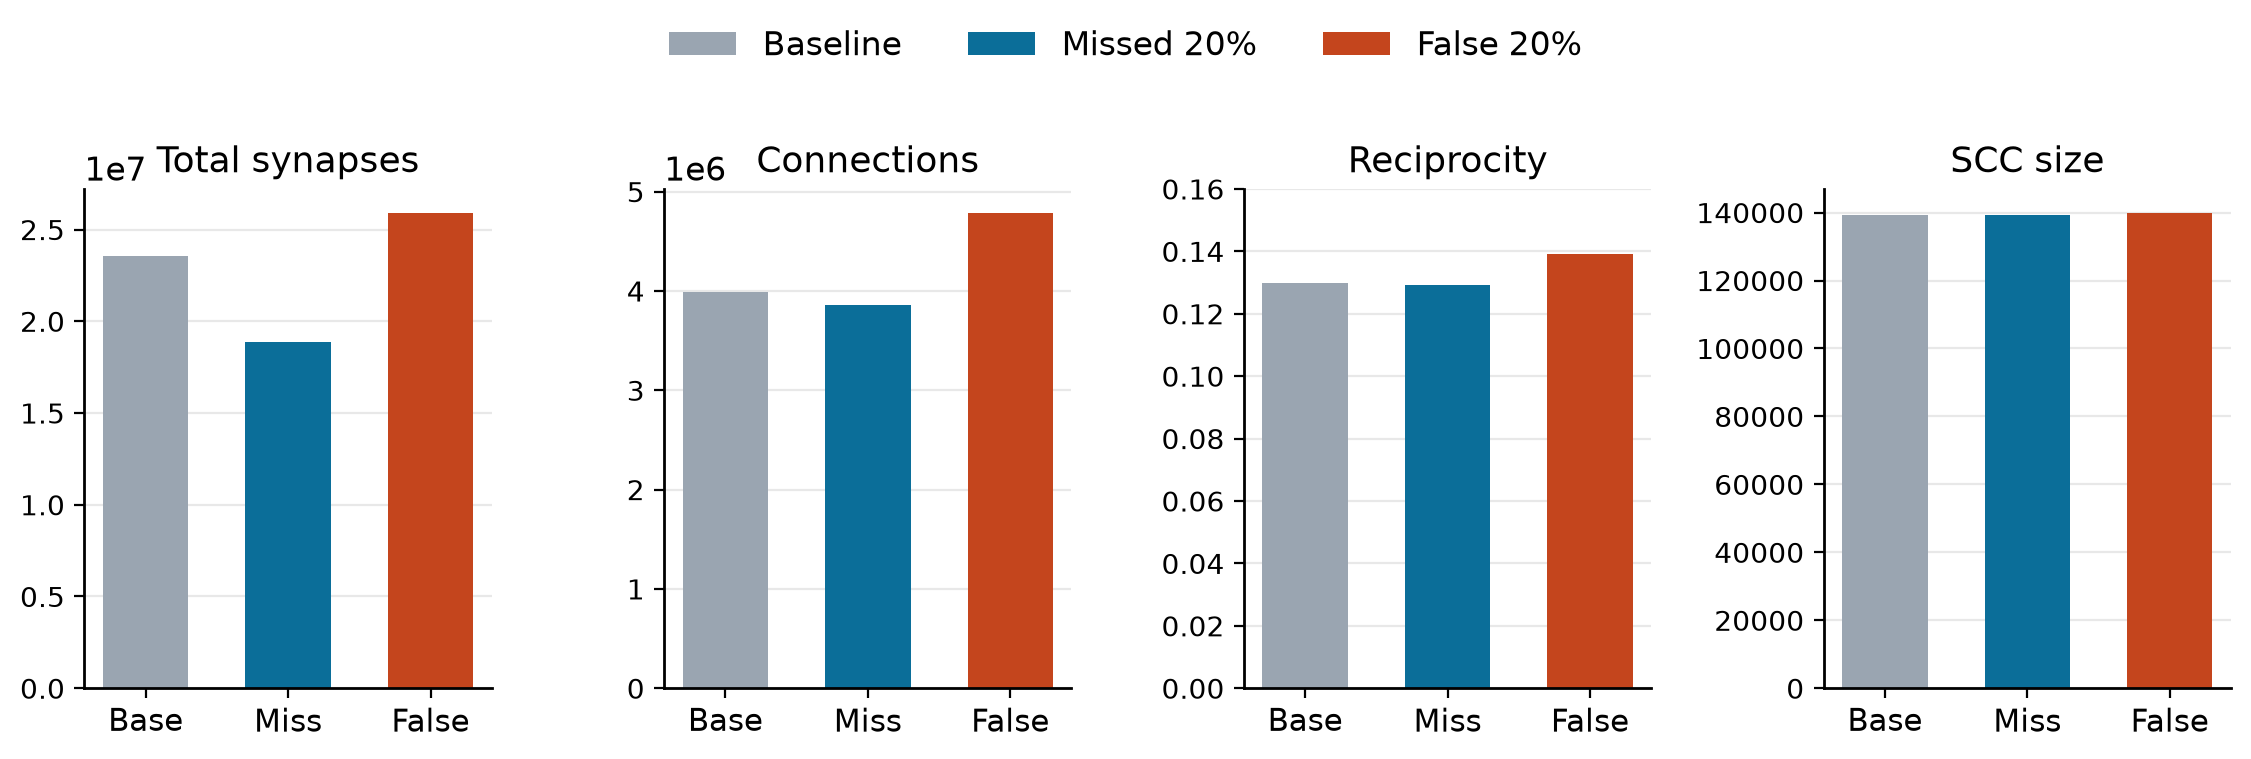
\includegraphics[width=0.86\textwidth]{fig_snapshot20}

\vskip2pt
\footnotesize
Baseline (gray) vs.\ 20\% missed (blue) vs.\ 20\% false (orange).
Note the plain (non-scientific) tick labels and honest zero-based scales.
\takeaway{Synapses shrink by a fifth under missed; edges grow by a fifth
under false.  Reciprocity and SCC size move only a few tenths of a percent.}
\end{frame}

% ============================================================================
% Slide 14 — Result 6: sensitivity ranking
% ============================================================================
\begin{frame}{Result 6: What Degrades First? --- Sensitivity Ranking}
\begin{columns}[c]
  \begin{column}{0.60\textwidth}
    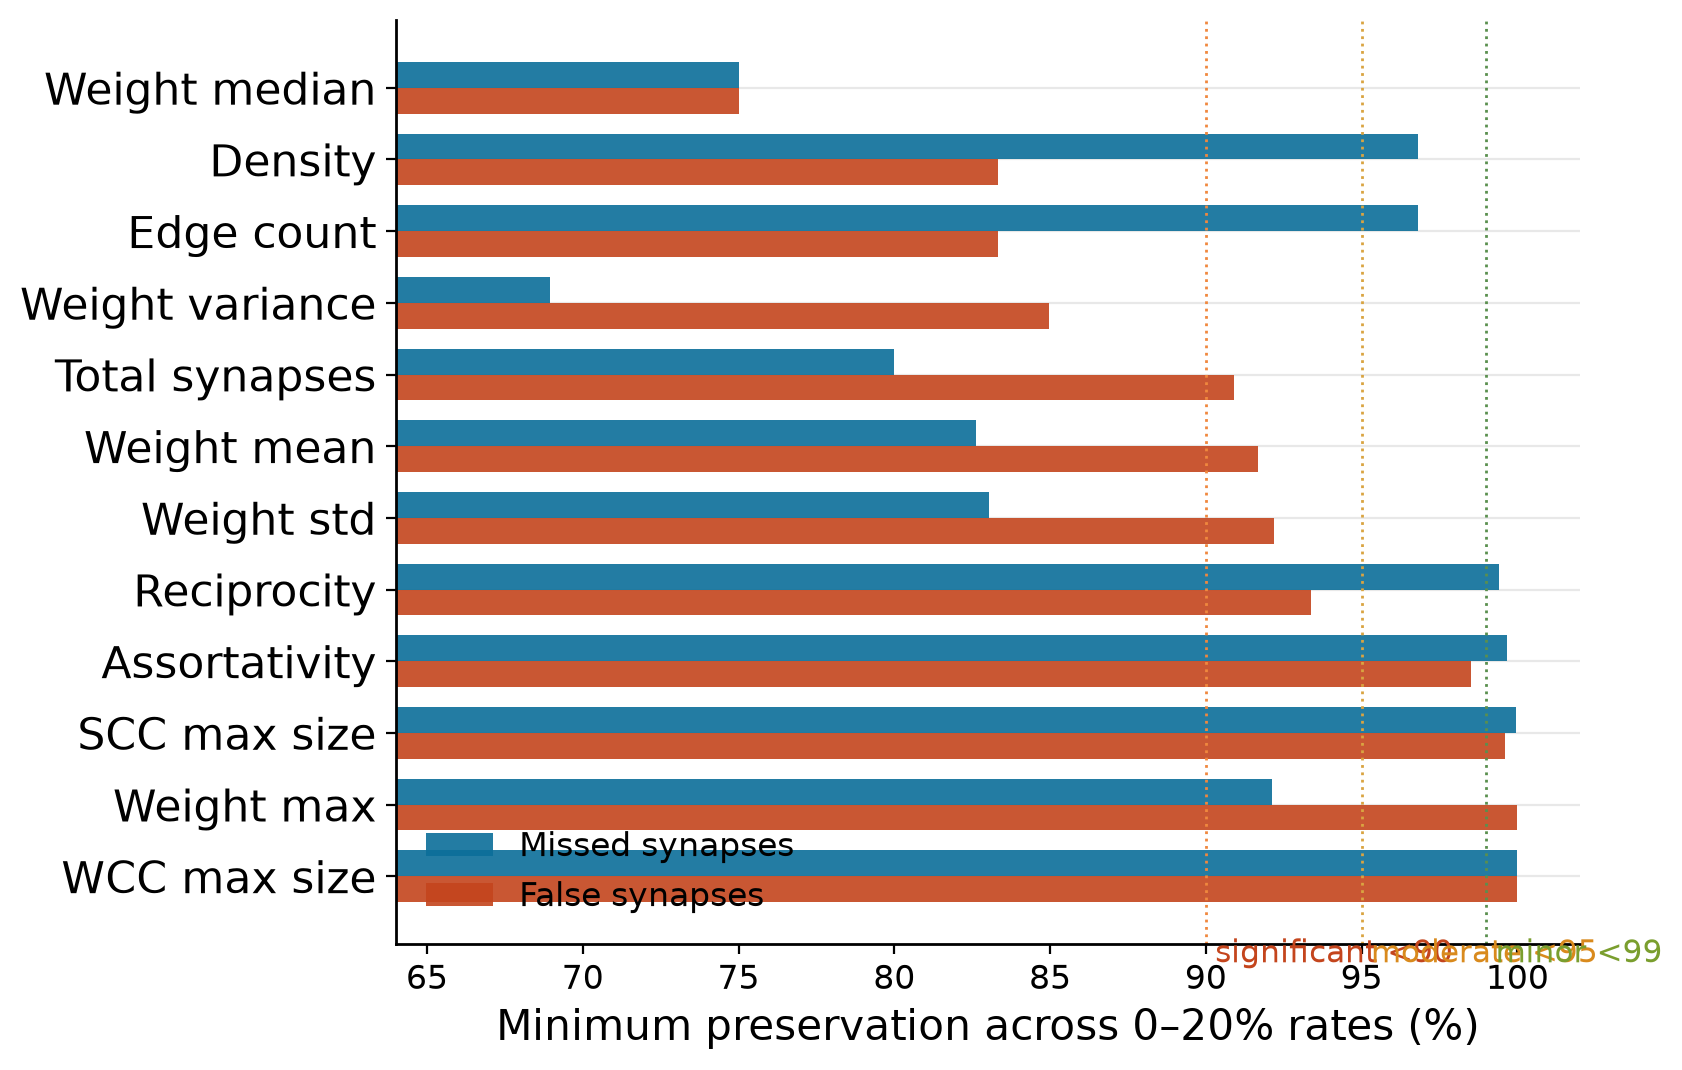
\includegraphics[width=\textwidth]{fig_ranking}
  \end{column}
  \begin{column}{0.38\textwidth}
    \footnotesize
    \begin{itemize}
      \item \textbf{Missed:} weight statistics degrade first --- variance
            68.9\%, median 75.0\%, synapses 80.0\%.
      \item \textbf{False:} edge count / density degrade first --- 83.3\%.
      \item Connectivity, reciprocity, assortativity: all $\ge$93\%.
      \item Threshold guides: significant $<$90\%, moderate $<$95\%, minor $<$99\%.
    \end{itemize}
  \end{column}
\end{columns}
\takeaway{The synaptic layer erodes first under missed synapses; the edge
layer erodes first under false synapses.  Global wiring is last to move.}
\end{frame}

% ============================================================================
% Slide 15 — Result 7: category preservation
% ============================================================================
\begin{frame}{Result 7: Preservation by Biological Category at 20\%}
\begin{columns}[c]
  \begin{column}{0.60\textwidth}
    \includegraphics[width=\textwidth]{fig_category20}
  \end{column}
  \begin{column}{0.38\textwidth}
    \scriptsize\setlength{\tabcolsep}{5pt}
    \renewcommand{\arraystretch}{1.2}
    \begin{tabular}{@{}llcc@{}}
      \toprule
      \textbf{Category} & \textbf{N} & \textbf{Missed} & \textbf{False}\\
      \midrule
      Structural Topology & 3 & 97.9\% & 88.9\%\\
      Synaptic Properties & 7 & 83.1\% & 90.7\%\\
      Connectivity & 2 & 100.0\% & 99.8\%\\
      Network Organization & 2 & 99.5\% & 95.9\%\\
      \bottomrule
    \end{tabular}
    \par\vspace{6pt}
    \footnotesize
    Unweighted mean of member-metric preservation scores at the 20\% rate.
  \end{column}
\end{columns}
\takeaway{Category-level view confirms the ranking: synaptic statistics and
structural topology are the sensitive layers; connectivity is untouched.}
\end{frame}

% ============================================================================
% Slide 16 — Comparison table
% ============================================================================
\begin{frame}{Comparison: Missed vs.\ False at 20\% Error}
\begin{columns}[c]
  \begin{column}{0.55\textwidth}
    \scriptsize\renewcommand{\arraystretch}{1.5}\setlength{\tabcolsep}{8pt}
    \begin{tabular}{@{}lrr@{}}
      \toprule
      \textbf{Metric @20\%} & \textbf{Missed} & \textbf{False}\\
      \midrule
      Total synapses & $-20.0\%$ & $+10.0\%$\\
      Edges & $-3.2\%$ & $+20.0\%$\\
      Reciprocity & $-0.6\%$ & $+7.1\%$\\
      SCC giant & $-0.05\%$ & $+0.40\%$\\
      PageRank corr. & 0.9975 & 0.9833\\
      Top-$k$ overlap & 0.970 & 0.892\\
      In-degree KS & 0.0052 & 0.0758\\
      \bottomrule
    \end{tabular}
  \end{column}
  \begin{column}{0.43\textwidth}
    \begin{block}{Same nominal rate $\rightarrow$ different fingerprints}
      \footnotesize
      Missed synapses \emph{deflate} the synapse pool while leaving edges
      and topology intact.
    \end{block}
    \begin{block}{}
      \footnotesize
      False synapses \emph{inflate} the edge count and distort degree
      distributions --- the more damaging of the two.
    \end{block}
  \end{column}
\end{columns}
\end{frame}

% ============================================================================
% Slide 17 — Reliability
% ============================================================================
\begin{frame}{Reliability of the Results}
\begin{columns}[T]
  \begin{column}{0.55\textwidth}
    \footnotesize
    \begin{itemize}
      \item \textbf{5 seeded trials} per rate $\times$ 10 rates $\times$ 2
            models.
      \item \textbf{Tight spread:} total-synapse $\sigma$ is only
            $\approx$0.01\% of the mean at 20\%.
      \item \textbf{Deterministic false edges:} injected edges reproduce
            exactly ($\sigma = 0$); missed trials agree to within
            $\approx$0.01\%.
      \item \textbf{Monotone primary trends} (synapses, edges, KS) across all
            ten rates --- no flips.
      \item \textbf{Consistent status labels} across trials
            (Preserved $\ge$99\% / Minor $\ge$95\% / Moderate $\ge$90\% /
            Significant $<$90\%).
    \end{itemize}
  \end{column}
  \begin{column}{0.43\textwidth}
    \begin{block}{Spread @20\% --- $\sigma$/mean (rel.)}
      \renewcommand{\arraystretch}{1.4}
      \begin{tabular}{@{}lll@{}}
        \toprule
        \textbf{Metric} & \textbf{Missed} & \textbf{False}\\
        \midrule
        Total synapses & $\pm$0.009\% & $\pm$0.005\%\\
        Edge count & $\pm$0.005\% & $\pm$0.000\%\\
        SCC giant & $\pm$0.010\% & $\pm$0.006\%\\
        \bottomrule
      \end{tabular}
    \end{block}
  \end{column}
\end{columns}
\end{frame}

% ============================================================================
% Slide 18 — Conclusions
% ============================================================================
\begin{frame}{Conclusions}
\begin{block}{Direct, measurable effects}
  \footnotesize
  Missed synapses remove synapses \emph{exactly} in proportion to the rate
  ($-20.0\%$ at 20\%); false synapses add edges \emph{exactly} in proportion
  ($+20.0\%$).  These are the most sensitive quantities measured.
\end{block}
\begin{block}{Topology is highly robust}
  \footnotesize
  Giant component and node count survive to $>$99\% even at 20\% error ---
  the coarse wiring plan is barely disturbed (PageRank correlation $\ge$0.98).
\end{block}
\begin{block}{False synapses are the more disruptive model}
  \footnotesize
  At equal nominal rates they distort degree distributions 6--14$\times$ more,
  erode hub ranking (top-$k$ 0.89 vs.\ 0.97) and raise reciprocity by $+7\%$.
\end{block}
\begin{block}{Error signatures are separable}
  \footnotesize
  Missed synapses \emph{deflate} synaptic statistics; false synapses
  \emph{inflate} the graph --- weak edges dilute weights without hubs.
\end{block}
\end{frame}

% ============================================================================
% Slide 19 — Summary / takeaway
% ============================================================================
\begin{frame}{Summary}
\centering
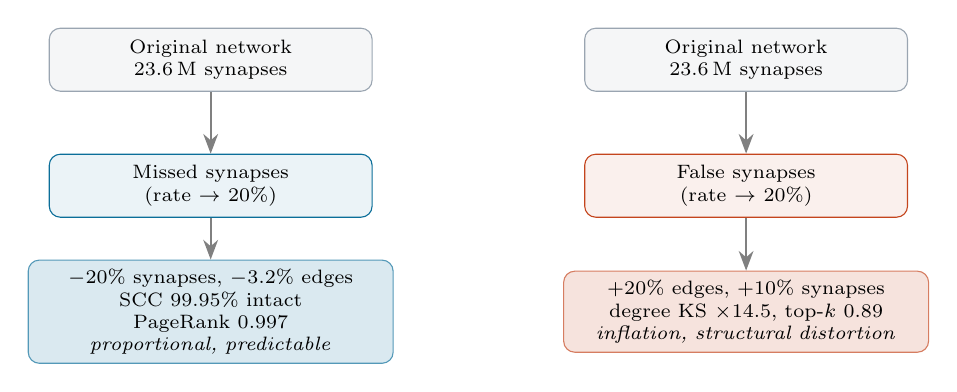
\begin{tikzpicture}[
  lane/.style={rounded corners=4pt, minimum width=4.1cm, minimum height=0.8cm,
               font=\scriptsize, draw, align=center},
  arr/.style={-{Stealth[length=2.5mm]}, thick, color=gray}
]
  \node[lane, draw=baselinec, fill=baselinec!10] (m0) at (0,0) {Original network\\ 23.6\,M synapses};
  \node[lane, draw=accent, fill=accent!8] (m1) at (0,-1.6) {Missed synapses\\ (rate $\rightarrow$ 20\%)};
  \node[lane, draw=accent!70, fill=accent!15, text width=4.4cm] (m2) at (0,-3.2)
        {$-20\%$ synapses, $-3.2\%$ edges\\ SCC 99.95\% intact\\ PageRank 0.997\\ \emph{proportional, predictable}};
  \draw[arr] (m0) -- (m1);
  \draw[arr] (m1) -- (m2);
  \node[lane, draw=baselinec, fill=baselinec!10] (f0) at (6.8,0) {Original network\\ 23.6\,M synapses};
  \node[lane, draw=accentb, fill=accentb!8] (f1) at (6.8,-1.6) {False synapses\\ (rate $\rightarrow$ 20\%)};
  \node[lane, draw=accentb!70, fill=accentb!15, text width=4.4cm] (f2) at (6.8,-3.2)
        {$+20\%$ edges, $+10\%$ synapses\\ degree KS $\times$14.5, top-$k$ 0.89\\ \emph{inflation, structural distortion}};
  \draw[arr] (f0) -- (f1);
  \draw[arr] (f1) -- (f2);
\end{tikzpicture}

\vskip6pt
\begin{beamercolorbox}[rounded=true,sep=6pt,wd=\textwidth]{block body}
  {\scriptsize\color{navy}\textbf{Takeaway:} reconstruction errors degrade
  synaptic statistics first --- global wiring stays intact.  False-positive
  errors are consistently more disruptive than missed synapses at the same
  rate.}
\end{beamercolorbox}
\end{frame}

\end{document}
